\documentclass[a4paper,11pt]{article}
\usepackage{graphicx}      % include figures
\usepackage{amsmath}       % math formulas
\usepackage{hyperref}      % clickable links and references
\usepackage{caption}       % custom captions 

\title{Optimization of Energy Generation Using Multiple Sources}
\author{Your Name}
\date{\today}

\begin{document}

\maketitle

\begin{abstract}
This report details the optimization of power generation across various energy sources (wind, solar, nuclear, and gas) based on hourly demand. The project was conducted using Python for optimization and LaTeX for documentation.
\end{abstract}

\section{Introduction}
Provide an introduction to your problem, goals, and objectives here.

\section{Methodology}
Describe the optimization problem setup, including the mathematical model, cost functions, and constraints.

\subsection{Objective Function}
The objective function used to minimize the total cost of generation is:
\[
\text{Cost} = C_1 P_1 + C_2 P_2 + C_3 P_3 + C_4 P_4
\]
Where:
- \(C_1, C_2, C_3, C_4\) are the cost coefficients for nuclear, wind, solar, and gas, respectively.
- \(P_1, P_2, P_3, P_4\) are the power generated by each source.

\section{Results}
You can include the plots generated in `visualization.py` here:

\begin{figure}[h!]
    \centering
    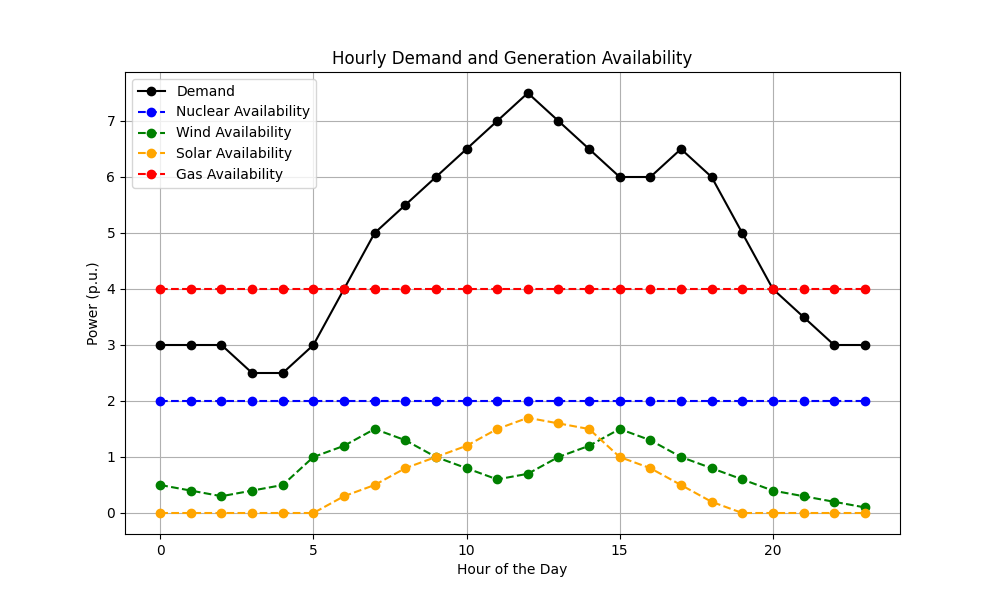
\includegraphics[width=0.8\textwidth]{figures/demand_vs_availability.png}
    \caption{Hourly demand vs generation availability}
    \label{fig:demand_availability}
\end{figure}

\begin{figure}[h!]
    \centering
    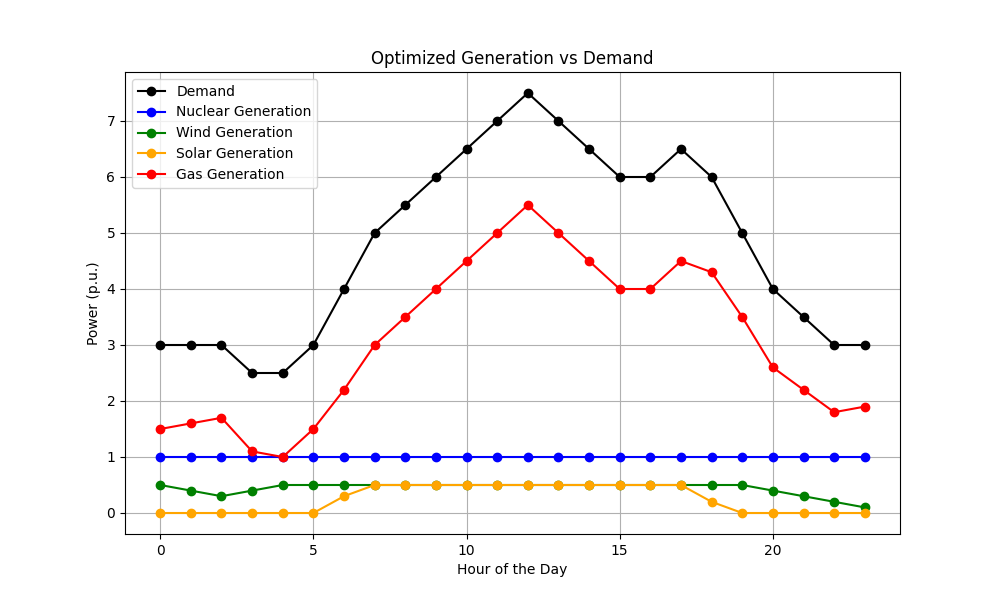
\includegraphics[width=0.8\textwidth]{figures/optimized_generation_vs_demand.png}
    \caption{Optimized generation vs demand}
    \label{fig:optimized_generation}
\end{figure}

\section{Conclusion}
Summarize your findings and any potential improvements for the future.

\bibliographystyle{plain}
\bibliography{bibliography}

\end{document}